\subsection{LASSO}\label{apen:lasso}

LASSO is a categorized procedure within the set of penalized regressions. Penalized Least Squares is a punishment procedure that adds to the OLS regression a component that penalizes weak coefficients. The Penalty Least Squares estimator is obtained through

\begin{align*}
	\widehat{\boldsymbol{\beta}}(\lambda)=\underset{\boldsymbol{\beta} \in \mathcal{B}}{\arg \min }\left[\sum_{i=1}^n\left(Y_i-\boldsymbol{\beta}^{\prime} \boldsymbol{X}_i\right)^2+\sum_{j=1}^p p_\lambda\left(\left|\beta_j\right| ; \boldsymbol{\alpha}, \text { data }\right)\right]
\end{align*}

where $p_\lambda\left(\left|\beta_j\right| ; \boldsymbol{\alpha}, \text{data}\right)$ is a non-negative penalty function indexed by the regularization parameter $\lambda$ and could rely on both the data and additional hyperparameters. For example,

\begin{itemize}
	\item Ridge
	
	$p_\lambda\left(\left|\beta_j\right| ; \boldsymbol{\alpha}\right.$, data $)=\lambda\left|\beta_j\right|^2$
	\item LASSO
	
	$p_\lambda\left(\left|\beta_j\right| ; \boldsymbol{\alpha}\right.$, data $)=\lambda\left|\beta_j\right|$
	\item LASSO and Ridge combined
	
	$p_\lambda\left(\left|\beta_j\right| ; \boldsymbol{\alpha}\right.$, data $)=\alpha \lambda\left|\beta_j\right|+(1-\alpha) \lambda\left|\beta_j\right|^2$
\end{itemize}

The regularization parameter $\lambda$ controls the number of parameters in the model. If $\lambda = \infty$, then no parameters enter the model, and if $\lambda = 0$, then the parameters are simply OLS estimators.



% FIGURES
\newpage
\subsection{Figures}

\begin{figure}[H]
\caption{Number of stocks in each Database}
\centering
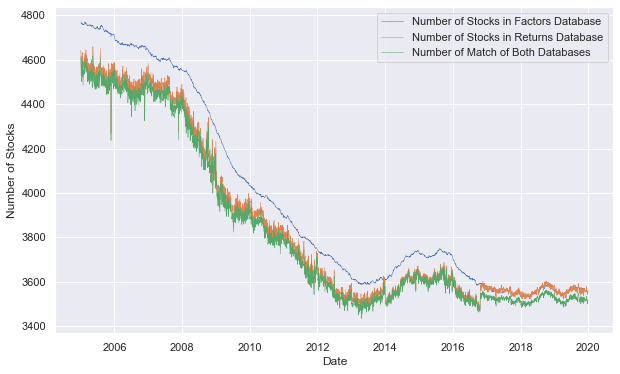
\includegraphics[scale=.73]{../../output/figures/match.png}
\label{fig:match}
\end{figure}


% TABLES
%\newpage
%\subsection{Tables}
%
%\begin{table}[H]
%\caption{}
%\centering
%\begin{threeparttable}
%%\input{../../output/}
%\end{threeparttable}
%\label{tab:}
%\end{table}






%% PORTUGUESE VERSION
%
%O LASSO é um procedimento categorizado dentro do conjunto de regressões penalizadas. O Penalized Least Squares é um procedimento de estimação que adiciona ao OLS um componente que penaliza os coeficientes fracos. O estimador de Penalized Least Squares é obtido através
%
%\begin{align*}
%	\widehat{\boldsymbol{\beta}}(\lambda)=\underset{\boldsymbol{\beta} \in \mathcal{B}}{\arg \min }\left[\sum_{i=1}^n\left(Y_i-\boldsymbol{\beta}^{\prime} \boldsymbol{X}_i\right)^2+\sum_{j=1}^p p_\lambda\left(\left|\beta_j\right| ; \boldsymbol{\alpha}, \text { data }\right)\right]
%\end{align*}
%
%onde $p_\lambda\left(\left|\beta_j\right| ; \boldsymbol{\alpha}, \text{data}\right)$ é uma função penalidade não negativa indexada pelo parâmetro de regularização $\lambda$ e poderia depender tanto dos dados quanto de hiper-parâmetros adicionais. Por exemplo,
%
%\begin{itemize}
%	\item Ridge
%	
%	$p_\lambda\left(\left|\beta_j\right| ; \boldsymbol{\alpha}\right.$, data $)=\lambda\left|\beta_j\right|^2$
%	\item LASSO
%	
%	$p_\lambda\left(\left|\beta_j\right| ; \boldsymbol{\alpha}\right.$, data $)=\lambda\left|\beta_j\right|$
%	\item LASSO e Ridge combinado
%	
%	$p_\lambda\left(\left|\beta_j\right| ; \boldsymbol{\alpha}\right.$, data $)=\alpha \lambda\left|\beta_j\right|+(1-\alpha) \lambda\left|\beta_j\right|^2$
%\end{itemize}
%
%O parâmetro de regularização $\lambda$ controla o número de parâmetros no modelo. Se $\lambda = \infty$, então nenhum parâmetro entra no modelo, e se $\lambda = 0$, então os parâmetros são simplesmente estimadores OLS.

